%%
%% getstart.tex -- Flight Gear documentation: The FlightGear Manual
%% Chapter file
%%
%% Written by Michael Basler, started September 1998.
%%
%% Copyright (C) 2002 Michael Basler
%%
%%
%% This program is free software; you can redistribute it and/or
%% modify it under the terms of the GNU General Public License as
%% published by the Free Software Foundation; either version 2 of the
%% License, or (at your option) any later version.
%%
%% This program is distributed in the hope that it will be useful, but
%% WITHOUT ANY WARRANTY; without even the implied warranty of
%% MERCHANTABILITY or FITNESS FOR A PARTICULAR PURPOSE.  See the GNU
%% General Public License for more details.
%%
%% You should have received a copy of the GNU General Public License
%% along with this program; if not, write to the Free Software
%% Foundation, Inc., 675 Mass Ave, Cambridge, MA 02139, USA.
%%
%% $Id: flight.tex,v 0.5 0.6 2002/09/09 michael
%% (Log is kept at end of this file)

%%%%%%%%%%%%%%%%%%%%%%%%%%%%%%%%%%%%%%%%%%%%%%%%%%%%%%%%%%%%%%%%%%%%%%%%%%%%%%%%
%%%%%%%%%%%%%%%
\iflanguage{english}{
\chapter{In-flight: All about instruments, keystrokes and menus}
}{}
\iflanguage{french}{
\chapter{En vol : tout sur les instruments, les raccourcis clavier et les menus}
}{}
\label{flight}
%%%%%%%%%%%%%%%%%%%%%%%%%%%%%%%%%%%%%%%%%%%%%%%%%%%%%%%%%%%%%%%%%%%%%%%%%%%%%%%%
%%%%%%%%%%%%%%%
\iflanguage{english}{
\markboth{\thechapter.\hspace*{1mm} FLIGHT}{\thesection\hspace*{1mm} KEYBOARD
CONTROLS}
}{}
\iflanguage{french}{
\markboth{\thechapter.\hspace*{1mm} EN VOL}{\thesection\hspace*{1mm} CONTROLES CLAVIER}
}{}

\iflanguage{english}{
The following is a description of the main systems for controlling the
program and piloting the plane. It is assumed that the reader is already
familiar with flying, possibly from experience on other simulators. If you are
completely new to flying, the tutorials in section \ref{tutorials} are a better
resource for learning to fly using FlightGear{}.

A short leaflet showing the standard keys and designed to be printed can be found at
}{}
\iflanguage{french}{
Voici une description des principaux syst\`{e}mes de contr\^{o}le du programme et
de pilotage de l'avion. On suppose que le lecteur est d\'{e}j\`{a} familiaris\'{e} avec le vol, peut-
\^{e}tre grace \`{a} de l'exp\'{e}rience acquise sur d'autres simulateurs. Si vous \^{e}tes un vrai
d\'{e}butant, les tutoriels de la section \ref{tutorials} sont plus appropri\'{e}s pour vous apprendre
\`{a} voler avec FlightGear.

Un petit livret, destin\'{e} \`{a} \^{e}tre imprim\'{e}, et contenant une liste des touches, est disponible
\`{a} l'adresse :
}{}

\medskip
\web{http://www.flightgear.org/Docs/FGShortRef.pdf}.
\medskip

\noindent
\iflanguage{english}{
A reference to most of the keyboard controls can be found under the Help menu in the simulator.
}{}
\iflanguage{french}{
Une r\'{e}f\'{e}rence \`{a} la plupart des contr\^{o}les du clavier se trouve dans le menu Aide
du simulateur.
}{}

%%%%%%%%%%%%%%%%%%%%%%%%%%%%%%%%%%%%%%%%%%%%%%%%%%%%%%%%%%%%%%%%%%%%%%%%%%%%%%%%
%%%%%%%%%%%%%%%
\iflanguage{english}{
\section{Starting the engine}\index{engine!starting}
}{}
\iflanguage{french}{
\section{D\'{e}marrer le moteur}\index{moteur!d\'{e}marrer}
}{}
%%%%%%%%%%%%%%%%%%%%%%%%%%%%%%%%%%%%%%%%%%%%%%%%%%%%%%%%%%%%%%%%%%%%%%%%%%%%%%%%
%%%%%%%%%%%%%%%

\iflanguage{english}{
Depending on the type of aircraft, you may have to start the engine(s) before you can
go flying. The instructions below are generic. Check the aircraft help or aircraft tutorials
for more specific instructions.

Once you've started the engine, you should check whether the \Index{parking brake}s are engaged.
If so, press the `B' key to release them.
}{}
\iflanguage{french}{
Suivant le type d'a\'{e}ronef, vous pouvez avoir \`{a} d\'{e}marrer le(s) moteur(s) avant
de pouvoir voler. Les instructions ci-dessous sont g\'{e}n\'{e}riques. Consultez l'aide de l'a\'{e}ronef ou les
tutoriels de l'avion pour obtenir des instructions plus sp\'{e}cifiques.

Une fois le moteur d\'{e}marr\'{e}, vous devez v\'{e}rifier si les \Index{freins de parking}
sont serr\'{e}s. Si c'est le cas, l\^{a}chez-les en appuyant sur la touche 'B'.
}{}

\iflanguage{english}{
\subsection{Piston Aircraft}\index{engine!starting!piston}
}{}
\iflanguage{french}{
\subsection{Moteur \`{a} pistons}\index{moteur!d\'{e}marrage!pistons}
}{}

\iflanguage{english}{
For piston-engined aircraft, the magnetos are controlled by the `\{' and `\}' keys. On most aircraft, the starter is engaged using
the `s' key. On multi-engined aircraft you can select which engines to control. Use `\~' to select all the engines at once. Most
magnetos have 4 positions - OFF, LEFT, RIGHT and BOTH. So, to start the selected engine, press the `\}' key three times, then hold
down `s'.

Note that the starting procedure for powerful WWII-era fighter aircraft is often more complex. See the aircraft help for details.
}{}
\iflanguage{french}{
Pour les a\'{e}ronefs disposant d'un moteur \`{a} pistons, les magn\'{e}tos sont control\'{e}s par les
touches `\{' et `\}'. Sur la plupart des a\'{e}ronefs, le d\'{e}marreur s'actionne en appuyant sur la
touche `s'. Sur les a\'{e}ronefs multi-moteurs, vous pouvez choisir quel moteur contr\^{o}ler. Utilisez
`\~' pour s\'{e}lectionner tous les moteurs \`{a} la fois. La plupart des magn\'{e}tos ont 4 positions - OFF, LEFT, RIGHT et BOTH.
Ainsi, pour d\'{e}marrer le moteur s\'{e}lectionn\'{e}, appuyez 3 fois sur la touche `\}', puis maintenez la touche `s'
enfonc\'{e}e jusqu'au d\'{e}marrage.

Notez que la proc\'{e}dure de d\'{e}marrage est souvent plus complexe pour les puissant avions de chasse de la seconde guerre mondiale. Consultez l'aide de l'avion pour avoir plus de d\'{e}tails.
}{}

\iflanguage{english}{
\subsection{Turboprop Aircraft}\index{engine!starting!turboprop}
}{}
\iflanguage{french}{
\subsection{A\'{e}ronefs \`{a} turbopropulseurs}\index{moteur!d\'{e}marrage!turbopropulseurs}
}{}

\iflanguage{english}{
Starting a turbo-prop engine generally requires simply moving the condition lever from Off to Idle, using 'm'.
}{}
\iflanguage{french}{
Le d\'{e}marrage d'un moteur turbopropuls\'{e} ne n\'{e}cessite g\'{e}n\'{e}ralement que de d\'{e}placer le levier
de commande de \textit{Off} \`{a} \textit{Idle}, en appuyant sur la touche 'm'.
}{}

\iflanguage{english}{
\subsection{Jet Aircraft}\index{engine!starting!jet}
}{}
\iflanguage{french}{
\subsection{A\'{e}ronefs \`{a} r\'{e}action}\index{moteur!d\'{e}marrage!avion \`{a} r\'{e}action}
}{}

\iflanguage{english}{
Starting a jet aircraft is significantly more complex, and the controls vary between different aircraft.
}{}
\iflanguage{french}{
Le d\'{e}marrage d'un a\'{e}ronef \`{a} r\'{e}action est bien plus complexe, et les contr\^{o}les varient selon l'appareil.
}{}

\begin{enumerate}
\iflanguage{english}{
\item Set cutoff ON
\item Engage the starter
\item Once the engines spools up to approximately 5\% N1, set cutoff OFF
\item Disengage the starter once the engine has reached operational speed.
}{}
\iflanguage{french}{
\item Placer l'interrupteur g\'{e}n\'{e}ral (\textit{cutoff}) sur la position ON.
\item Actionner le d\'{e}marreur (\textit{starter}).
\item Lorsque les moteurs approchent des 5\% N1, remettez le \textit{cutoff} sur OFF.
\item Coupez le d\'{e}marreur une fois que le moteur a atteint sa vitesse op\'{e}rationnelle.
}{}
\end{enumerate}

%%%%%%%%%%%%%%%%%%%%%%%%%%%%%%%%%%%%%%%%%%%%%%%%%%%%%%%%%%%%%%%%%%%%%%%%%%%%%%%%
%%%%%%%%%%%%%%%
\iflanguage{english}{
\section{Keyboard controls}\index{keyboard controls}
}{}
\iflanguage{french}{
\section{Contr\^{o}les clavier}\index{contr\^{o}les clavier}
}{}
%%%%%%%%%%%%%%%%%%%%%%%%%%%%%%%%%%%%%%%%%%%%%%%%%%%%%%%%%%%%%%%%%%%%%%%%%%%%%%%%
%%%%%%%%%%%%%%%

\iflanguage{english}{
While \Index{joystick}s, \Index{yoke}s and \Index{rudder pedals} are supported,
you can fly \FlightGear{} using the keyboard alone or in conjunction with a mouse,
described below. However you control the aircraft, you will need to use the keyboard
for at least some controls.

These key bindings\index{keybindings!configuration} are not hard-coded, but
user-adjustable. You can check and change these setting via the file
\texttt{keyboard.xml}\index{keyboard.xml} which can be found in the main
\FlightGear{} directory. This is a human-readable plain ASCII file.
Although it's perhaps not the best idea for beginners to modify this file,
more advanced users will find it useful to change key bindings according to
their wishes, e.g. to match other simulators.
}{}
\iflanguage{french}{
Bien que les \Index{joystick}s, les \Index{volant}s et les \Index{p\'{e}dales de palonnier} soient pris en charge,
vous pouvez choisir de voler avec \FlightGear{} avec l'usage du clavier, seul ou utilis\'{e} conjointement
avec la souris, comme d\'{e}crit ci-dessous. Mais, quelle que soit la fa\c{c}on dont vous contr\^{o}lez votre
a\'{e}ronef, vous serez oblig\'{e} d'utiliser le clavier, ne serait-ce que pour quelques actions.

L'attribution de fonctions \`{a} des touches (\index{raccourcis clavier!configuration} ne sont pas cod\'{e}s en durs,
mais ajustables par l'utilisateur. Vous pouvez contr\^{o}ler et modifier ces param\`{e}tres via le fichier \texttt{keyboard.xml},
qui peut \^{e}tre trouv\'{e} dans le r\'{e}pertoire  principal de \FlightGear{}. C'est un fichier texte au format
ASCII lisible par un humain. Bien que les modifications \`{a} ce fichier ne soient pas recommand\'{e}es aux d\'{e}butants,
des utilisateurs plus aguerris peuvent trouver utile de modifier l'attribution de fonctions aux touches, au gr\'{e}
de leurs souhaits, par exemple pour les faire correspondre \`{a} ce qui peut \^{e}tre trouv\'{e} sur d'autres simulateurs.
}{}

\iflanguage{english}{
\subsection{Aircraft controls}\index{keyboard controls!primary}
}{}
\iflanguage{french}{
\subsection{Contr\^{o}les de l'a\'{e}ronef}\index{contr\^{o}les clavier!base}
}{}

\iflanguage{english}{
In order to have full control of the plane during flight using the keyboard you should ensure that
\texttt{\Index{NumLock}} is on, and the \FlightGear{} window is in focus. The following keys control
the primary aircraft surfaces.
}{}
\iflanguage{french}{
Pour parvenir \`{a} contr\^{o}ler pleinement votre avion en utilisant votre clavier pendant la phase de vol, vous devriez
vous assurer que \texttt{\Index{NumLock}} est activ\'{e}, et que la fen\^{e}tre \FlightGear{} est active. Les touches suivantes
assurent le contr\^{o}le les surfaces de base de l'a\'{e}ronef.
}{}

\medskip
\centerline{%%
%% tab2.tex -- Flight Gear documentation: The FlightGear Manual
%% Keyboard controls table 1/Main controls
%%
%% Written by Michael Basler, started September 1998.
%%
%% Copyright (C) 2002 Michael Basler
%%
%%
%% This program is free software; you can redistribute it and/or
%% modify it under the terms of the GNU General Public License as
%% published by the Free Software Foundation; either version 2 of the
%% License, or (at your option) any later version.
%%
%% This program is distributed in the hope that it will be useful, but
%% WITHOUT ANY WARRANTY; without even the implied warranty of
%% MERCHANTABILITY or FITNESS FOR A PARTICULAR PURPOSE.  See the GNU
%% General Public License for more details.
%%
%% You should have received a copy of the GNU General Public License
%% along with this program; if not, write to the Free Software
%% Foundation, Inc., 675 Mass Ave, Cambridge, MA 02139, USA.
%%
%% $Id: tab1.tex,v 0.6 2002/09/09 michael
%% (Log is kept at end of this file)
%%%%%%%%%%%%%%%%%%%%%%%%%%%%%%%%%%%%%%%%%%%%%%%%%%%%%%%%%%%%%%%%%%%%%%%%%%%%%%%%%%%%%%%%%%%%%%%%
\begin{tabular}{|l|l|}\hline
\IfLanguageName{english}{
  Key      &  Action\\\hline
 9 / 3     &  Throttle\index{throttle}\\
 4 / 6     &  Aileron\index{aileron}\\
 8 / 2     &  Elevator\index{elevator}\\
 0 / Enter &  Rudder\index{rudder}\\
 5         &  Center aileron/elevator/rudder\\
 7 / 1     &  Elevator \Index{trim}\\\hline
}{}
\IfLanguageName{french}{
  Touche      &  Action\\\hline
 9 / 3     &  Commande des gaz\index{gaz}\\
 4 / 6     &  Aileron\index{aileron}\\
 8 / 2     &  Gouverne de profondeur\index{gouverne de profondeur}\\
 0 / Entr\'{e}e &  gouverne de direction\index{gouverne de direction}\\
 5         &  Centrage des ailerons/gouverne de profondeur/direction\\
 7 / 1     &  Trim de la gouverne de profondeur \Index{trim}\\\hline
}{}
\IfLanguageName{italian}{
  Pulsante/i      &  Azione\\\hline
 9 / 3     &  Manetta (Throttle)\index{manetta}\index{throttle}\\
 4 / 6     &  Alettoni\index{Alettoni}\\
 8 / 2     &  Elevatore (timone di coda)\index{Elevatore}\\
 0 / Invio &  Timone di direzione\index{gouverne de direction}\\
 5         &  Centra alettoni, timone di coda e di direzione\\
 7 / 1     &  Regola il trim \Index{trim}\\\hline
}{}

\end{tabular}

%% revision 0.5 2002/02/15 michael
%% Initial revision
}
\iflanguage{english}{
Table 1: \textit{Primary aircraft controls}
}{}
\iflanguage{french}{
Tableau 1 : \textit{Contr\^{o}les de base de l'a\'{e}ronef}
}{}
\medskip

\iflanguage{english}{
The following keys control the engines\index{engine controls}.
}{}
\iflanguage{french}{
Les touches suivantes contr\^{o}lent les moteurs\index{contr\^oles moteurs}.
}{}

\medskip
\centerline{%%
%% tab7.tex -- Flight Gear documentation: The FlightGear Manual
%% Keyboard controls table 6/Engine related controls
%%
%% Written by Michael Basler, started September 1998.
%%
%% Copyright (C) 2002 Michael Basler
%%
%%
%% This program is free software; you can redistribute it and/or
%% modify it under the terms of the GNU General Public License as
%% published by the Free Software Foundation; either version 2 of the
%% License, or (at your option) any later version.
%%
%% This program is distributed in the hope that it will be useful, but
%% WITHOUT ANY WARRANTY; without even the implied warranty of
%% MERCHANTABILITY or FITNESS FOR A PARTICULAR PURPOSE.  See the GNU
%% General Public License for more details.
%%
%% You should have received a copy of the GNU General Public License
%% along with this program; if not, write to the Free Software
%% Foundation, Inc., 675 Mass Ave, Cambridge, MA 02139, USA.
%%
%% $Id: tab6.tex,v 0.6 2002/09/09 michael
%% (Log is kept at end of this file)
%%%%%%%%%%%%%%%%%%%%%%%%%%%%%%%%%%%%%%%%%%%%%%%%%%%%%%%%%%%%%%%%%%%%%%%%%%%%%%%%%%%%%%%%%%%%%%%%
\begin{tabular}{|l|l|}\hline
  \ifchinese
  按键   &    操作\\\hline
  !     &    选择第一号发动机\\
  @     &    选择第二号发动机\\
  \#    &    选择第三号发动机\\
  \$    &    选择第四号发动机\\
  $\sim$$ &  选择所有发动机\\\hline
  \{    &    减少所选发动机的磁电机档位\\
  \}    &    增加所选发动机的磁电机档位\\
  s     &    为所选的发动机点火启动\\
  M / m &    贫油/富油所选发动机的油气混合比\\
  N / n &    减少/增加所选发动机的螺旋桨转速 \\\hline
  \fi
\iffalse
\IfLanguageName{english}{
Key      &  Action\\ \hline
   !     & Select 1st engine\\
   @	   & Select 2nd engine\\
  \#     & Select 3rd engine\\
  \$     & Select 4th engine\\
  $\sim$ & Select all engines\\\hline
  \{     & Decrease magneto on selected engine\\
  \}     & Increase magneto on selected engine\\
   s     & Fire starter on selected engine(s)\\
  M / m  & Lean/Enrich selected engine mixture\\
  N / n  & Decrease/Increase selected propeller RPM\\\hline
}{}
\fi
\IfLanguageName{french}{
Touche     &  Action\\ \hline
   !     & S\'{e}l\'{e}ctionne le premier moteur\\
   @	 & S\'{e}l\'{e}ctionne le deuxi\`{e}me moteur\\
  \#     & S\'{e}l\'{e}ctionne le troisi\`{e}me moteur\\
  \$     & S\'{e}l\'{e}ctionne le quatri\`{e}me moteur\\
  $\sim$ & S\'{e}l\'{e}ctionne tous les moteurs\\\hline
  \{     & D\'{e}cr\'{e}mente le magn\'{e}to sur le moteur s\'{e}lectionn\'{e}\\
  \}     & Incr\'{e}mente le magn\'{e}to sur le moteur s\'{e}lectionn\'{e}\\
   s     & D\'{e}marrage du/des moteur(s) s\'{e}lectionn\'{e}(s)\\
  M / m  & Appauvrir/Enrichir le m\'{e}lange du moteur s\'{e}lectionn\'{e}\\
  N / n  & Diminue/Augmente le nombre de tours par minute du moteur s\'{e}lectionn\'{e}\\\hline
}{}
\IfLanguageName{italian}{
Pulsante/i &  Azione\\ \hline
   !     & Seleziona il 1\textdegree{} motore\\
   @	   & Seleziona il 2\textdegree{} motore\\
  \#     & Seleziona il 3\textdegree{} motore\\
  \$     & Seleziona il 4\textdegree{} motore\\
  $\sim$ & Seleziona tutti i motori\\\hline
  \{     & Diminuisce la forza dei magneti sui motori selezionati\\
  \}     & Aumenta la forza dei magneti sui motori selezionati\\
   s     & Avvia i(l) motore/i selezionato/i\\
  M / m  & Impoverisce/Arricchisce la miscela del motore selezionato\\
  N / n  & Diminuisce/Aumenta il passo dell'elica del motore selezionato\\\hline
}{}
\end{tabular}

%% revision 0.5 2002/02/15 michael
%% Initial revision
}
\iflanguage{english}{
Table 2: \textit{Engine control keys\index{keyboard controls!engine}}
}{}
\iflanguage{french}{
Tableau 2 : \textit{Touches de contr\^{o}le du moteur\index{contr\^{o}les clavier!moteur}}
}{}

\medskip

\iflanguage{english}{
The following keys control secondary aircraft systems.
}{}
\iflanguage{french}{
Les touches suivantes contr\^{o}lent les syst\`{e}mes secondaires de l'a\'{e}ronef.
}{}

\medskip
\centerline{%%
%% tab8.tex -- Flight Gear documentation: The FlightGear Manual
%% Keyboard controls table 7/Miscellaneous
%%
%% Written by Michael Basler, started September 1998.
%%
%% Copyright (C) 2002 Michael Basler
%%
%%
%% This program is free software; you can redistribute it and/or
%% modify it under the terms of the GNU General Public License as
%% published by the Free Software Foundation; either version 2 of the
%% License, or (at your option) any later version.
%%
%% This program is distributed in the hope that it will be useful, but
%% WITHOUT ANY WARRANTY; without even the implied warranty of
%% MERCHANTABILITY or FITNESS FOR A PARTICULAR PURPOSE.  See the GNU
%% General Public License for more details.
%%
%% You should have received a copy of the GNU General Public License
%% along with this program; if not, write to the Free Software
%% Foundation, Inc., 675 Mass Ave, Cambridge, MA 02139, USA.
%%
%% $Id: tab7.tex,v 0.5 2002/15/02 michael
%% (Log is kept at end of this file)
%%%%%%%%%%%%%%%%%%%%%%%%%%%%%%%%%%%%%%%%%%%%%%%%%%%%%%%%%%%%%%%%%%%%%%%%%%%%%%%%%%%%%%%%%%%%%%%%
\begin{tabular}{|l|l|}\hline
  \ifchinese
  按键       &    操作\\\hline
  b         &    启用所有\Index{刹车}\\
  , / .     &    启用左右刹车\\
            &    (用于\Index{差动刹车})\\
  l         &    切换\Index{尾轮锁定}\\
  B         &    切换停留刹车 \index{刹车}\index{停留刹车}\\
  g / G     &    收起/放下起落架 \index{机轮}\index{起落架}\\
  空格       &    按键通话(PTT)\\
  - / \_    &    多人飞行时文字聊天菜单/输入\\
  $[$ / $]$ &    收起/放下\Index{襟翼}\\
  j / k     &    收起/张开\Index{扰流板}\\
  CTRL-B    &    切换\Index{减速板}\\\hline
  \fi
\iffalse
\IfLanguageName{english}{
Key           &  Action\\\hline
  b           & Apply  all \Index{brakes}\\
  , / .       & Apply left/right brake \\
              & (useful for \Index{differential braking})\\
  l           & Toggle \Index{tail-wheel lock}\\
  B           & Toggle parking brake \index{brakes}\index{parking brake}\\
  g/G         & Raise/lower landing gear\index{gear}\index{landing gear}\\
  Space       & Push To Talk (PTT)\\
  - / \_      & MP text chat menu/entry\\
  $[$ / $]$   & Retract/extend \Index{flaps}\\
  j / k       & Retract/extend \Index{spoilers}\\
  Ctrl-B      & Toggle \Index{speed brakes}\\ \hline
}{}
\fi
\IfLanguageName{french}{
Touche        &  Action\\\hline
  b           & Appliquer tous les \Index{freins}\\
  , / .       & Appliquer le frein gauche/droit\\
              & (utile pour le \Index{freinage diff\'{e}rentiel})\\
  l           & Active le \Index{verrouillage de la roue de queue}\\
  B           & Active le frein de parking \index{freins}\index{freins de parking}\\
  g/G         & Monter/descendre le train d'atterrissage\index{train d'atterrissage}\index{train d'atterrissage}\\
  Espace      & Appuyez pour parler (Push To Talk, PTT)\\
  - / \_      & Entr\'{e}e/menu du clavardage clavier du mode multijoueurs\\
  $[$ / $]$   & Rentre/d\'{e}ploie les \Index{volets}\\
  j / k       & Rentre/d\'{e}ploie les \Index{a\'{e}rofreins}\\
  Ctrl-B      & Active les \Index{freins de vitesse}\\ \hline
}{}
\IfLanguageName{italian}{
Pulsante/i     &  Azione\\\hline
  b           & Applica tutti i \Index{freni} (tenere premuto)\\
  , / .       & Applica/Toglie il freno di sinistra/destra \\
  l           & Mette/Toglie il \Index{blocco delle ruote di coda}\\
  B           & Toglie/Mette i \Index{freni di parcheggio}\\
  g/G         & Alza/Abbassa il carrello d'atterraggio\index{carrello d'atterraggio}\\
  Space       & Tenendolo premuto si parla usando FGCom (PTT)\\
  - / \_      & Comandano la chat scritta\\
  $[$ / $]$   & Ritrae/Estende i \Index{flaps}\\
  j / k       & Ritrae/Estende i \Index{deflettori}\\
  Ctrl-B      & Applica/Toglie gli \Index{aerofreni}\\ \hline
}{}
\end{tabular}

%% revision 0.5 2002/02/15 michael
%% Initial revision
}
\iflanguage{english}{
Table 3: \textit{Secondary aircraft controls\index{keyboard controls!aircraft}}
}{}
\iflanguage{french}{
Tableau 3 : \textit{Contr\^oles secondaires de l'a\'{e}ronef\index{contr\^{o}les clavier!a\'{e}ronef}}
}{}

\medskip

\iflanguage{english}{
Autopilot controls are as follows.
}{}
\iflanguage{french}{
Les contr\^{o}les du pilote automatique sont les suivants.
}{}

\medskip
\centerline{%%
%% tab5.tex -- Flight Gear documentation: Installation and Getting Started
%% Keyboard controls table 4/autopilot controls
%%
%% Written by Michael Basler, started September 1998.
%%
%% Copyright (C) 2002 Michael Basler
%%
%%
%% This program is free software; you can redistribute it and/or
%% modify it under the terms of the GNU General Public License as
%% published by the Free Software Foundation; either version 2 of the
%% License, or (at your option) any later version.
%%
%% This program is distributed in the hope that it will be useful, but
%% WITHOUT ANY WARRANTY; without even the implied warranty of
%% MERCHANTABILITY or FITNESS FOR A PARTICULAR PURPOSE.  See the GNU
%% General Public License for more details.
%%
%% You should have received a copy of the GNU General Public License
%% along with this program; if not, write to the Free Software
%% Foundation, Inc., 675 Mass Ave, Cambridge, MA 02139, USA.
%%
%% $Id: tab4.tex,v 0.6 2002/09/09 michael
%% (Log is kept at end of this file)
%%%%%%%%%%%%%%%%%%%%%%%%%%%%%%%%%%%%%%%%%%%%%%%%%%%%%%%%%%%%%%%%%%%%%%%%%%%%%%%%%%%%%%%%%%%%%%%%
\begin{tabular}{|l|l|}\hline
 Key              &         Action\\\hline
    Ctrl + A      &         Altitude hold\index{altitude hold} toggle on/off\\
    Ctrl + G      &         Follow glide slope 1 toggle on/off\\
    Ctrl + H      &         Heading hold\index{heading hold} toggle on/off\\
    Ctrl + N      &         Follow NAV 1 radial toggle on/off\\
    Ctrl + S      &         Autothrottle\index{autothrottle} toggle on/off\\
    Ctrl + T      &         Terrain follow toggle on/off\\
    Ctrl + U      &         Add 1000 ft. to your altitude (emergency)\\
    Enter		      &         Increase autopilot heading\\
    F6 		    		&         Toggle autopilot target:\\
                  &         current heading/waypoint\\
    F11           &         Autopilot altitude dialog\\
    F12           &         Autopilot heading dialog\\\hline
\end{tabular}

%% revision 0.5 2002/02/15 michael
%% Initial revision}
\iflanguage{english}{
Table 4: \textit{Autopilot controls\index{keyboard controls! autopilot}}
}{}
\iflanguage{french}{
Tableau 4 : \textit{Contr\^les du pilote automatique\index{contr\^{o}les clavier!pilote automatique}}
}{}
\medskip

\iflanguage{english}{
\subsection{Simulator controls}\index{keyboard controls!simulator controls}
}{}
\iflanguage{french}{
\subsection{Contr\^{o}les du simulateur}\index{contr\^{o}les clavier!contr\^{o}les du simulateur}
}{}

\iflanguage{english}{
To change the \Index{view direction}, you must de-activate \texttt{NumLock}. The available controls are as follows:
}{}
\iflanguage{french}{
Pour changer la \Index{direction de la vue}, vous devez d\'{e}sactiver \texttt{NumLock}. Les contr\^{o}les disponibles sont
les suivants :
}{}
\medskip

\centerline{%%
%% tab3.tex -- Flight Gear documentation: The FlightGear Manual
%% Keyboard controls table 2/View directions
%%
%% Written by Michael Basler, started September 1998.
%%
%% Copyright (C) 2002 Michael Basler
%%
%%
%% This program is free software; you can redistribute it and/or
%% modify it under the terms of the GNU General Public License as
%% published by the Free Software Foundation; either version 2 of the
%% License, or (at your option) any later version.
%%
%% This program is distributed in the hope that it will be useful, but
%% WITHOUT ANY WARRANTY; without even the implied warranty of
%% MERCHANTABILITY or FITNESS FOR A PARTICULAR PURPOSE.  See the GNU
%% General Public License for more details.
%%
%% You should have received a copy of the GNU General Public License
%% along with this program; if not, write to the Free Software
%% Foundation, Inc., 675 Mass Ave, Cambridge, MA 02139, USA.
%%
%% $Id: tab2.tex,v 0.6 2002/09/09 michael
%% (Log is kept at end of this file)
%%%%%%%%%%%%%%%%%%%%%%%%%%%%%%%%%%%%%%%%%%%%%%%%%%%%%%%%%%%%%%%%%%%%%%%%%%%%%%%%%%%%%%%%%%%%%%%%
\begin{tabular}{|c|l|}\hline
\iflanguage{english}{
   Numpad Key  &  View direction\index{view directions}\\\hline
    Shift-8  & Forward\\
    Shift-7  & Left/forward\\
    Shift-4  & Left\\
    Shift-1  & Left/back\\
    Shift-2  & Back\\
    Shift-3  & Right/back\\
    Shift-6  & Right\\
    Shift-9  & Right/forward\\\hline
}{}
\iflanguage{french}{
   Touche pav\'{e} num\'{e}rique & Angle de vue\index{angle de vue}\\\hline
    Shift-8  & Vers l'avant\\
    Shift-7  & Avant/Gauche\\
    Shift-4  & Gauche\\
    Shift-1  & Arri\`{e}re/Gauche\\
    Shift-2  & Arri\`{e}re\\
    Shift-3  & Arri\`{e}re/Droit\\
    Shift-6  & Droit\\
    Shift-9  & Avant/Droit\\\hline
}{}
\end{tabular}

%% revision 0.5 2002/02/15 michael
%% Initial revision
}
\iflanguage{english}{
Table 5: \textit{View directions\index{keyboard controls! view}}
}{}
\iflanguage{french}{
Tableau 5 : \textit{Directions de la vue\index{contr\^{o}les clavier! vue}}
}{}
\medskip

\iflanguage{english}{
Additionally, the following keys allow you to control the display:
}{}
\iflanguage{french}{
De plus, les touches suivantes vous permettent de contr\^{o}ler l'affichage :
}{}
\medskip

\noindent
\centerline{%%
%% tab4.tex -- Flight Gear documentation: Installation and Getting Started
%% Keyboard controls table 3/Additional view options
%%
%% Written by Michael Basler, started September 1998.
%%
%% Copyright (C) 2002 Michael Basler (pmb@epost.de)
%%
%%
%% This program is free software; you can redistribute it and/or
%% modify it under the terms of the GNU General Public License as
%% published by the Free Software Foundation; either version 2 of the
%% License, or (at your option) any later version.
%%
%% This program is distributed in the hope that it will be useful, but
%% WITHOUT ANY WARRANTY; without even the implied warranty of
%% MERCHANTABILITY or FITNESS FOR A PARTICULAR PURPOSE.  See the GNU
%% General Public License for more details.
%%
%% You should have received a copy of the GNU General Public License
%% along with this program; if not, write to the Free Software
%% Foundation, Inc., 675 Mass Ave, Cambridge, MA 02139, USA.
%%
%% $Id: tab3.tex,v 0.6 2002/09/09 michael
%% (Log is kept at end of this file)
%%%%%%%%%%%%%%%%%%%%%%%%%%%%%%%%%%%%%%%%%%%%%%%%%%%%%%%%%%%%%%%%%%%%%%%%%%%%%%%%%%%%%%%%%%%%%%%%
\begin{tabular}{|l|l|}\hline
 Key              &         Action\\\hline
 P                &    Toggle \Index{instrument panel} on/off \\
 c                &    Toggle3D/2D cockpit
 											 \index{2D cockpit} (if both are available)
 											 \index{3D cockpit}\index{cockpit}\\
 s                &    Cycle panel style full/mini\\
 Shift-F5/F6      &    Shift the panel in y direction\\
 Shift-F7/F8      &    Shift the panel in x direction\\
 Shift-F3					&    Read a panel from a property list\\
 i/I              &    Minimize/maximize HUD              \\
 h/H              &    Change color  of HUD/toggle HUD off\\
                  &    forward/backward      \\   \hline
  x/X             &    Zoom in/out\\
   v              &    Cycle \Index{view modes} (pilot, chase, tower)\\ \hline
   W              &    Toggle \Index{full screen mode} on/off (3dfx only)\\
   z/Z            &    Change \Index{visibility} (fog)  forward/backward \\
   F8             &    Toggle fog on/off\\
   F2			 				& 	 Refresh Scenery tile cache\\
   F4			 				& 	 Force Lighting update\\
   F9             &    Toggle texturing on/off\\
   F10      			&    Toggle menu on/off\\ \hline   
 \end{tabular}

%% revision 0.5 2002/02/15 michael
%% Initial revision}
\iflanguage{english}{
Table 6: \textit{Display options\index{display options}\index{keyboard controls! display}}
}{}
\iflanguage{french}{
Tableau 6 : \textit{Options d'affichage\index{Options d'affichage}\index{contr\^{o}les clavier! affichage}}
}{}
\medskip

\iflanguage{english}{
Finally, the following general simulator controls are available.
}{}
\iflanguage{french}{
Enfin, les contr\^{o}les g\'{e}n\'{e}raux suivants du simulateur sont disponibles.
}{}

\medskip
\centerline{%%
%% tab8.tex -- Flight Gear documentation: The FlightGear Manual
%% Keyboard controls table 7/Miscellaneous
%%
%% Written by Michael Basler, started September 1998.
%%
%% Copyright (C) 2002 Michael Basler
%%
%%
%% This program is free software; you can redistribute it and/or
%% modify it under the terms of the GNU General Public License as
%% published by the Free Software Foundation; either version 2 of the
%% License, or (at your option) any later version.
%%
%% This program is distributed in the hope that it will be useful, but
%% WITHOUT ANY WARRANTY; without even the implied warranty of
%% MERCHANTABILITY or FITNESS FOR A PARTICULAR PURPOSE.  See the GNU
%% General Public License for more details.
%%
%% You should have received a copy of the GNU General Public License
%% along with this program; if not, write to the Free Software
%% Foundation, Inc., 675 Mass Ave, Cambridge, MA 02139, USA.
%%
%% $Id: tab7.tex,v 0.5 2002/15/02 michael
%% (Log is kept at end of this file)
%%%%%%%%%%%%%%%%%%%%%%%%%%%%%%%%%%%%%%%%%%%%%%%%%%%%%%%%%%%%%%%%%%%%%%%%%%%%%%%%%%%%%%%%%%%%%%%%
\begin{tabular}{|l|l|}\hline
  \ifchinese
  按键       &    操作\\\hline
  b         &    启用所有\Index{刹车}\\
  , / .     &    启用左右刹车\\
            &    (用于\Index{差动刹车})\\
  l         &    切换\Index{尾轮锁定}\\
  B         &    切换停留刹车 \index{刹车}\index{停留刹车}\\
  g / G     &    收起/放下起落架 \index{机轮}\index{起落架}\\
  空格       &    按键通话(PTT)\\
  - / \_    &    多人飞行时文字聊天菜单/输入\\
  $[$ / $]$ &    收起/放下\Index{襟翼}\\
  j / k     &    收起/张开\Index{扰流板}\\
  CTRL-B    &    切换\Index{减速板}\\\hline
  \fi
\iffalse
\IfLanguageName{english}{
Key           &  Action\\\hline
  b           & Apply  all \Index{brakes}\\
  , / .       & Apply left/right brake \\
              & (useful for \Index{differential braking})\\
  l           & Toggle \Index{tail-wheel lock}\\
  B           & Toggle parking brake \index{brakes}\index{parking brake}\\
  g/G         & Raise/lower landing gear\index{gear}\index{landing gear}\\
  Space       & Push To Talk (PTT)\\
  - / \_      & MP text chat menu/entry\\
  $[$ / $]$   & Retract/extend \Index{flaps}\\
  j / k       & Retract/extend \Index{spoilers}\\
  Ctrl-B      & Toggle \Index{speed brakes}\\ \hline
}{}
\fi
\IfLanguageName{french}{
Touche        &  Action\\\hline
  b           & Appliquer tous les \Index{freins}\\
  , / .       & Appliquer le frein gauche/droit\\
              & (utile pour le \Index{freinage diff\'{e}rentiel})\\
  l           & Active le \Index{verrouillage de la roue de queue}\\
  B           & Active le frein de parking \index{freins}\index{freins de parking}\\
  g/G         & Monter/descendre le train d'atterrissage\index{train d'atterrissage}\index{train d'atterrissage}\\
  Espace      & Appuyez pour parler (Push To Talk, PTT)\\
  - / \_      & Entr\'{e}e/menu du clavardage clavier du mode multijoueurs\\
  $[$ / $]$   & Rentre/d\'{e}ploie les \Index{volets}\\
  j / k       & Rentre/d\'{e}ploie les \Index{a\'{e}rofreins}\\
  Ctrl-B      & Active les \Index{freins de vitesse}\\ \hline
}{}
\IfLanguageName{italian}{
Pulsante/i     &  Azione\\\hline
  b           & Applica tutti i \Index{freni} (tenere premuto)\\
  , / .       & Applica/Toglie il freno di sinistra/destra \\
  l           & Mette/Toglie il \Index{blocco delle ruote di coda}\\
  B           & Toglie/Mette i \Index{freni di parcheggio}\\
  g/G         & Alza/Abbassa il carrello d'atterraggio\index{carrello d'atterraggio}\\
  Space       & Tenendolo premuto si parla usando FGCom (PTT)\\
  - / \_      & Comandano la chat scritta\\
  $[$ / $]$   & Ritrae/Estende i \Index{flaps}\\
  j / k       & Ritrae/Estende i \Index{deflettori}\\
  Ctrl-B      & Applica/Toglie gli \Index{aerofreni}\\ \hline
}{}
\end{tabular}

%% revision 0.5 2002/02/15 michael
%% Initial revision
}
\iflanguage{english}{
Table 7: \textit{General simulator controls.\index{keyboard controls! general}}
}{}
\iflanguage{french}{
Tableau 7 : \textit{Contr\^{o}les g\'{e}n\'{e}raux du simulateur.\index{contr\^{o}les clavier! g\'{e}n\'{e}ral}}
}{}
\medskip

\iflanguage{english}{
\subsection{Autopilot controls}\index{keyboard controls!autopilot}
}{}
\iflanguage{french}{
\subsection{Contr\^{o}les du pilote automatique}\index{contr\^{o}les clavier!pilote automatique}
}{}

\iflanguage{english}{
\FlightGear{} supports two types of \Index{autopilot} - a \Index{generic autopilot}
that works with all aircraft (even those that would not normally have an autopilot),
and aircraft-specific autopilots that are controlled from within the cockpit.

The generic autopilot is controlled via the following keys:
}{}
\iflanguage{french}{
\FlightGear{} prend en charge deux types de \Index{pilote automatique} - un \Index{pilote automatique g\'{e}n\'{e}rique},
qui fonctionne avec tous les a\'{e}ronefs (m\^{e}me ceux qui, en temps normal, n'auraient pas de pilote automatique), et des
pilotes automatiques sp\'{e}cifiques \`{a} un a\'{e}ronef en particulier et qui sont contr\^{o}l\'{e}s \`{a} partir du cockpit.

Le pilote automatique g\'{e}n\'{e}rique est contr\^{o}l\'{e} via les touches suivantes :
}{}

\medskip

\centerline{%%
%% tab5.tex -- Flight Gear documentation: Installation and Getting Started
%% Keyboard controls table 4/autopilot controls
%%
%% Written by Michael Basler, started September 1998.
%%
%% Copyright (C) 2002 Michael Basler
%%
%%
%% This program is free software; you can redistribute it and/or
%% modify it under the terms of the GNU General Public License as
%% published by the Free Software Foundation; either version 2 of the
%% License, or (at your option) any later version.
%%
%% This program is distributed in the hope that it will be useful, but
%% WITHOUT ANY WARRANTY; without even the implied warranty of
%% MERCHANTABILITY or FITNESS FOR A PARTICULAR PURPOSE.  See the GNU
%% General Public License for more details.
%%
%% You should have received a copy of the GNU General Public License
%% along with this program; if not, write to the Free Software
%% Foundation, Inc., 675 Mass Ave, Cambridge, MA 02139, USA.
%%
%% $Id: tab4.tex,v 0.6 2002/09/09 michael
%% (Log is kept at end of this file)
%%%%%%%%%%%%%%%%%%%%%%%%%%%%%%%%%%%%%%%%%%%%%%%%%%%%%%%%%%%%%%%%%%%%%%%%%%%%%%%%%%%%%%%%%%%%%%%%
\begin{tabular}{|l|l|}\hline
 Key              &         Action\\\hline
    Ctrl + A      &         Altitude hold\index{altitude hold} toggle on/off\\
    Ctrl + G      &         Follow glide slope 1 toggle on/off\\
    Ctrl + H      &         Heading hold\index{heading hold} toggle on/off\\
    Ctrl + N      &         Follow NAV 1 radial toggle on/off\\
    Ctrl + S      &         Autothrottle\index{autothrottle} toggle on/off\\
    Ctrl + T      &         Terrain follow toggle on/off\\
    Ctrl + U      &         Add 1000 ft. to your altitude (emergency)\\
    Enter		      &         Increase autopilot heading\\
    F6 		    		&         Toggle autopilot target:\\
                  &         current heading/waypoint\\
    F11           &         Autopilot altitude dialog\\
    F12           &         Autopilot heading dialog\\\hline
\end{tabular}

%% revision 0.5 2002/02/15 michael
%% Initial revision}
\noindent
\iflanguage{english}{
 Tab.\,6: \textit{Autopilot controls.\index{autopilot controls}}
}{}
\iflanguage{french}{
 Tableau\,6 : \textit{contr\^{o}les du pilote automatique.\index{contr\^{o}les du pilote automatique}}
}{}
\medskip

\iflanguage{english}{
\noindent Ctrl + T is especially interesting as it makes your aircraft behave
like a cruise missile, and follow the terrain. Ctrl + U might be handy in case
you feel you're just about to crash.

When the \Index{autopilot} is enabled, some of the numeric keypad keys function
differently and adjust the autopilot rather than the controls themselves:
}{}
\iflanguage{french}{
\noindent Ctrl + T est particuli\`{e}rement int\'{e}ssant car il va faire se comporter votre a\'{e}ronef comme un
missile de croisi\`{e}re, en effectuant un suivi de terrain. Ctrl + U peut \^{e}tre utile si vous sentez que vous
n'allez pas tadger \`{a} vous \'{e}craser.

Quand le \Index{pilote automatique} est activ\'{e}, certaines des touches du pav\'{e} num\'{e}rique fonctionnent diff\'{e}remment
et ajustent le pilote automatique au lieu des commandes de vol \`{a} proprement parler :
}{}

\medskip
\centerline{%%
%% tab6.tex -- Flight Gear documentation: Installation and Getting Started
%% Keyboard controls table 5/key actions for autopilot enabled
%%
%% Written by Michael Basler, started September 1998.
%%
%% Copyright (C) 2002 Michael Basler (pmb@epost.de)
%%
%%
%% This program is free software; you can redistribute it and/or
%% modify it under the terms of the GNU General Public License as
%% published by the Free Software Foundation; either version 2 of the
%% License, or (at your option) any later version.
%%
%% This program is distributed in the hope that it will be useful, but
%% WITHOUT ANY WARRANTY; without even the implied warranty of
%% MERCHANTABILITY or FITNESS FOR A PARTICULAR PURPOSE.  See the GNU
%% General Public License for more details.
%%
%% You should have received a copy of the GNU General Public License
%% along with this program; if not, write to the Free Software
%% Foundation, Inc., 675 Mass Ave, Cambridge, MA 02139, USA.
%%
%% $Id: tab5.tex,v 0.6 2002/09/09 michael
%% (Log is kept at end of this file)
%%%%%%%%%%%%%%%%%%%%%%%%%%%%%%%%%%%%%%%%%%%%%%%%%%%%%%%%%%%%%%%%%%%%%%%%%%%%%%%%%%%%%%%%%%%%%%%%
\begin{tabular}{|l|l|}\hline
 Key           &         Action\\\hline
    8 / 2      &         Altitude adjust\\
    0 / ,      &         Heading adjust\\
    9 / 3      &         Autothrottle adjust \\\hline
 \end{tabular}

%% revision 0.5 2002/02/15 michael
%% Initial revision}
\noindent
\iflanguage{english}{
 Tab.\,7: \textit{Additional Autopilot controls.}
}{}
\iflanguage{french}{
 Tab.\,7 : \textit{Contr\^{o}les additionnels du pilote automatique.}
}{}
\medskip

\iflanguage{english}{
Note that some keyboards use ``.'' instead of ``,''.
}{}
\iflanguage{french}{
Notez que certains claviers utilisent ``.'' au lieu de ``,''.
}{}

%%%%%%%%%%%%%%%%%%%%%%%%%%%%%%%%%%%%%%%%%%%%%%%%%%%%%%%%%%%%%%%%%%%%%%%%%%%%%%%%
%%%%%%%%%%%%%%%
\iflanguage{english}{
\section{Mouse-controlled actions\index{mouse, actions}\index{mouse}}
}{}
\iflanguage{french}{
\section{Actions contr\^{o}l\'{e}es par la souris\index{souris, actions}\index{souris}}
}{}
%%%%%%%%%%%%%%%%%%%%%%%%%%%%%%%%%%%%%%%%%%%%%%%%%%%%%%%%%%%%%%%%%%%%%%%%%%%%%%%%
%%%%%%%%%%%%%%%

\iflanguage{english}{
As well as selecting menu items and clicking on controls in the cockpit, your
mouse can be used for a variety of other valuable functions in \FlightGear{}.

There are three \Index{mouse modes}: Normal (the default), Control and View. You can
change between them by using the right mouse button.
}{}
\iflanguage{french}{
De m\^{e}me qu'elle permet de s\'{e}lectionner des \'{e}l\'{e}ments du menu ou de cliquer sur des commandes au sein du cockpit,
votre souris peut \'{e}galement \^{e}tre utilis\'{e}e dans \FlightGear{} \`{a} de nombreuses fins utiles.

Il y a trois \Index{modes souris} : Normal (par d\'{e}faut), Contr\^{o}le et Vue. Vous pouvez basculer de l'un \`{a} l'autre
en utilisant le bouton droit de la souris.
}{}

\iflanguage{english}{
\subsection{Normal mode}\index{mouse, normal}
}{}
\iflanguage{french}{
\subsection{Mode normal}\index{souris, normal}
}{}

\iflanguage{english}{
In normal mode, you can control the menus and the panel controls. This mode is indicated by
a normal arrow cursor.

To change a switch or toggle, simply click on it with the left or middle mouse button.

To change a knob on a radio or linear control such as the throttle, click on the left
hand side to decrease the value, and the right hand side to increase the value. Click
with the left mouse button to make a small adjustment, or the right button to make a
large one. Some controls, such as radios, also support using the mouse wheel.

Pressing Ctrl-C highlights the clickable hotspots and objects.
}{}
\iflanguage{french}{
En mode Normal, vous pouvez contr\^{o}ler les menus et les commandes du tableau de bord. L'activation de ce mode est
indiqu\'{e}e par un curseur disposant d'une fl\`{e}che normale.

Pour actionner un commutateur ou un interrupteur, cliquez simplement sur celui-ci avec le bouton gauche ou
milieu de la souris.

Pour faire tourner un bouton sur une radio ou une commande lin\'{e}aire comme la manette des gaz, cliquez sur le c\^{o}t\'{e}
gauche de celui-ci pour faire diminuer sa valeur, et sur le c\^{o}t\'{e} droit pour l'augmenter. Cliquez avec le
bouton gauche de la souris pour r\'{e}aliser de petits ajustements, avec le bouton droit pour des ajustements plus importants.
Certaines commandes, comme les radios, prennent \'{e}galement en charge la molette de la souris.

Un appui sur Ctrl-C illumine les zones et les objets cliquables.
}{}

\iflanguage{english}{
\subsection{Control mode}\index{mouse, control}
}{}
\iflanguage{french}{
\subsection{Mode contr\^{o}le}\index{souris, contr\^{o}le}
}{}

\iflanguage{english}{
In control mode you can control the aircraft flight controls by moving the mouse.
This mode is indicated by a cross-hair mouse cursor.

In this mode, moving the mouse left or right controls the ailerons and rolls the
aircraft. Moving the mouse forwards and or backwards controls the elevator and
changes the pitch of the aircraft.

Holding the left mouse button down changes the behaviour so that moving the
mouse left/right controls the rudder. Holding the middle mouse button down and
moving the mouse forwards/backwards controls the throttle.

Finally, the scroll-wheel may be used to set the elevator trim.

This mode is particularly useful if you do not have a joystick, as it provides much better
control of the aircraft than using the keyboard. If you intend to use the mouse to control
the aircraft regularly, it is recommended that you enabled auto-coordination, so the
ailerons are linked to the rudder. This can be done using \texttt{-$ $-enable-auto-coordination}
when lauching the simulator, or selecting auto-coordination from the launcher.
}{}
\iflanguage{french}{
En mode Contr\^{o}le, vous pouvez contr\^{o}ler les commandes de vol de l'a\'{e}ronef en bougeant la souris.
L'activation de ce mode est indiqu\'{e}e par la pr\'{e}sence d'un curseur de souris en forme de croix.

Dans ce mode, le d\'{e}placement de la souris vers la droite ou vers la gauche contr\^{o}le les
ailerons et le roulis de l'avion. La d\'{e}placer vers l'avant ou vers l'arri\`{e}re contr\^{o}le la
gouverne de profondeur et change l'inclinaison de l'avion.

Maintenir le bouton gauche appuy\'{e} tout en bougeant la souris vers la droite ou la gauche contr\^{o}le le
palonnier. Tenir appuy\'{e} le bouton du milieu tout en bougeant vers l'arri\`{e}re ou l'avant la souris
permet de contr\^{o}ler la manette des gaz.

Enfin, la molette peut \^{e}tre utilis\'{e}e pour param\'{e}trer le trim.

Ce mode est particuli\`{e}rement pratique si vous n'avez pas de joystick. On a ainsi un
bien meilleur contr\^{o}le de l'a\'{e}ronef qu'avec le clavier. Si vous avez l'intention de piloter
r\'{e}guli\`{e}rement votre avion avec la souris, il vous est recommand\'{e} d'activer l'auto-
coordination, qui solidarise ailerons et palonnier. Ceci peut \^{e}tre r\'{e}alis\'{e} en activant l'option
\texttt{-$ $-enable-auto-coordination}, ou en choisissant auto-coordination \`{a} partir de l'assistant.
}{}

\iflanguage{english}{
\subsection{View mode}\index{mouse, view}
}{}
\iflanguage{french}{
\subsection{Mode vue}\index{souris, vue}
}{}

\iflanguage{english}{
In view mode you can look around using the mouse. This mode is indicated by a double-headed
arrow cursor.

Simply moving the mouse pans and tilts your view in the current position. This is
particularly useful for looking around the cockpit, or out a side window. The
scroll-wheel can be used to zoom in or out. Clicking the left mouse button
resets the view back to its initial position, usually straight ahead.

Holding down the middle mouse button and moving the mouse allows you to move the viewpoint
itself left/right and up/down. Moving the mouse while both the middle button and Ctrl are
held down allows you to move the viewpoint forwards and backwards.
}{}
\iflanguage{french}{
En mode Vue, vous pouvez regarder autour de vous en utilisant la souris. L'activation de ce mode
est indiqu\'{e}e par la pr\'{e}sence d'un curseur de souris \`{a} double flèche.

Bouger simplement la souris vous permet de visualiser l'espace autour votre position actuelle. Ceci est
particuli\`{e}rement utile pour regarder autour du cockpit ou par une fen\^{e}tre lat\'{e}rale.
On peut utiliser la molette pour zoomer ou d\'{e}-zoomer. Cliquer sur le bouton gauche de la souris rempositionne
la vue \`{a} sa position initiale, en g\'{e}n\'{e}ral droit devant.

En maintenant appuy\'{e} le bouton du milieu de la souris tout en bougeant cette derni\`{e}re vous permet de
faire varier le point de vue vers la gauche/la droite et vers le haut/le bas. En bougeant la souris tout en
maintenant \`{a} la fois le bouton du milieu et la touche Ctrl enfonc\'{e}s vous permet de faire bouger le
point de vue vers l'avant et vers l'arri\`{e}re.
}{}

%%%%%%%%%%%%%%%%%%%%%%%%%%%%%%%%%%%%%%%%%%%%%%%%%%%%%%%%%%%%%%%%%%%%%%%%%%%%%%%%
%%%%%%%%%%%%%%%
\iflanguage{english}{
\section{Menu entries}\index{menu entries}
}{}
\iflanguage{french}{
\section{Entr\'{e}es du menu}\index{Entr\'{e}es du menu}
}{}
%%%%%%%%%%%%%%%%%%%%%%%%%%%%%%%%%%%%%%%%%%%%%%%%%%%%%%%%%%%%%%%%%%%%%%%%%%%%%%%%
%%%%%%%%%%%%%%%

\iflanguage{english}{
The menu bar provides access to a variety of options for the simulator and the aircraft.
Many aircraft have their own menu items, for changing their registration to automatically
starting their engines. These can be found at the end of the menu bar.

To display or hide the menu bar, press F10. You can also display the menu automatically
by moving your mouse to the top of the screen.

The menu bar provides the following menus and options.
}{}
\iflanguage{french}{
La barre de menu permet d'acc\'{e}der \`{a} diff\'{e}rentes options du simulateur et de l'a\'{e}ronef.
La plupart des avions ont leurs propres entr\'{e}es de menus, pour changer leur immatriculation
ou d\'{e}marrer automatiquement leurs moteurs. Ces \'{e}l\'{e}ments peuvent \^{e}tre trouv\'{e}s tout \`{a}
la fin de la barre de menu.
Pour afficher ou cacher la barre de menu, appuyez sur F10. Vous pouvez aussi afficher le menu automatiquement
en actionnant votre souris en haut de l'\'{e}cran.

La barre de menu propose les menus et options suivantes.
}{}

\begin{itemize}
\iflanguage{english}{
 \item \textbf{File}
 \begin{itemize}
 \item \textbf{Reset (Shift-Esc)} resets\index{reset flight} the flight to the selected starting
position. Comes in handy if you get lost or something goes wrong.
  \item \textbf{Screenshot (F3)} saves a screen shot\index{screenshot} as \\
  \texttt{fgfs-screen-XXX.jpg}.
  \item \textbf{Screenshot Directory} allows you to set the directory for \\
screenshots to be saved to.
  \item \textbf{Sound Configuration} configures the volume for various sound
channels, and whether they are heard outside the aircraft.
  \item \textbf{Quit (Esc)} exits\index{exit} the program.
}{}
\iflanguage{french}{
 \item \textbf{Fichier}
 \begin{itemize}
 \item \textbf{R\'{e}initialiser (Shift-Esc)} r\'{e}initialise \index{r\'{e}initialiser un vol} le vol \`{a} la position de d\'{e}marrage s\'{e}lectionn\'{e}e. Tr\`{e}s pratique si jamais vous \^{e}tes perdu ou que quelque chose tourne mal.
  \item \textbf{Capture d'\'{e}cran (F3)} sauvegarde une capture d'\'{e}cran\index{capture d'\'{e}cran} comme \texttt{fgfs-screen-XXX.jpg}.
  \item \textbf{R\'{e}pertoire des captures} vous permet de pr\'{e}ciser le r\'{e}pertoire o\`{u} les captures d'\'{e}cran seront  sauvegard\'{e}es.
  \item \textbf{Configuration du son} permet de configurer le volume pour diff\'{e}rents canaux sonores, et s'ils doivent \^{e}tre entendus en-dehors de l'a\'{e}ronef.
  \item \textbf{Quitter (Esc)} quitte\index{quitter} le programme.
}{}
 \end{itemize}

\iflanguage{english}{
 \item \textbf{View}\index{view}
 \begin{itemize}
  \item \textbf{Display Options} configures various display options, including whether the 2D panel, frame rate and chat messages are displayed.
  \item \textbf{Rendering Options} configures various graphical features. This allows you to trade eye-candy such as shadows, 3D clouds and specular reflections for frame-rate. To help you achieve a good balance, enable the ``Show Frame Rate'' option in the
Display Options menu, which will show the current frame-rate in frames-per-second in the bottom right of the screen.
  Most people find a frame-rate of around 20fps adequate for flying. The frame-rate is affected by the graphical features you have enabled, the current visibility (set by Z/z), the number of objects in view and their level of detail (LOD).
  \item \textbf{View Options} configures which views are enabled.
  \item \textbf{Cockpit View Options} configures the view within the cockpit, the pilot's head movement, black-out due
to high G, and redout due to negative G.
  \item \textbf{Adjust LOD Ranges} sets the range at which different levels of detail are displayed. This affects the textures and objects displayed in the simulator.
  \item \textbf{Adjust View Position} displays the current view offset.
  You can adjust this by dragging the dials. Alternatively you can make small adjustments   to your view-point using the mouse (see above).
  \item \textbf{Adjust HUD Properties} configures the Head Up Display (HUD) settings, such as transparency and whether anti-aliasing is used to display it.
 \item \textbf{Toggle Glide Slope Tunnel} displays a virtual tunnel to guide you down to the runway on a normal approach path. Useful if you are having difficulties setting up your approach for landing.
  \item \textbf{Instant Replay (Ctrl-R)} controls the instant replay feature - a good tool for checking your landings!
   \item \textbf{Stereoscopic View Options} configures stereoscopic display, using Red/Green glasses or other display methods.
\end{itemize}
}{}
\iflanguage{french}{
\item \textbf{Affichage}\index{Affichage}
 \begin{itemize}
  \item \textbf{Options d'affichage} permet de configurer diverses options d'affichage, notamment si le tableau de bord 2D, le taux de rafra\^{i}ssement d'images et les messages de clavardage sont affich\'{e}s.
  \item \textbf{Options de rendu} configure diverses fonctionnalit\'{e}s graphiques. Ceci vous permet de g\'{e}rer le compromis entre les effets visuels sympathiques, comme les ombres, les nuages 3D et les r\'{e}flexions sp\'{e}culaires et le taux de rafra\^{i}chissement des images. Pour vous permettre d'arriver \`{a} un compromis acceptable, l'activation de l'option ``Afficher le taux de rafra\^{i}chissement'' option dans le menu Options d'affichage, vous permettra de visualiser le taux d'images par seconde (\textit{frames per second, fps}) actuel dans l'angle inf\'{e}rieur droit de l'\'{e}cran. La plupart des personnes trouvent qu'un taux d'environ 20 fps est suffisant pour voler. Ce taux est d\'{e}pendant des fonctionnalit\'{e}s graphiques que vous avez activ\'{e}, la visibilit\'{e} du moment (param\'{e}tr\'{e} par Z/z), le nombre d'objets visibles et leur niveau de d\'{e}tails (\textit{Level Of Detail, LOD}).
  \item \textbf{Options de la vue} configure les vues activ\'{e}es.
  \item \textbf{Options d'affichage du cockpit} configure la vue au sein du cockpit, le mouvement de la t\^{e}te du pilote, le voile noir d\^{u} \`{a} la prise importante de G positifs et le voile rouge d\^{u} \`{a} la prise important de G n\'{e}gatifs.
  \item \textbf{Ajuster le niveau de d\'{e}tail} fixe la distance jusqu'\`{a} laquelle diff\'{e}rents niveaux de d\'{e}tails sont affich\'{e}s. Ceci affecte les textures et objets affich\'{e}s par le simulateur.
  \item \textbf{Ajuster la position de la vue} Affiche le d\'{e}calage de vue actuel. Vous pouvez ajuster cette valeur en d\'{e}pla\c{c}ant les contr\^{o}les. Sinon, vous pouvez r\'{e}aliser de petits ajustements de votre point de vue en utilisant la souris (voir ci-dessus).
  \item \textbf{Ajuster les propri\'{e}t\'{e}s du HUD} configure les param\`{e}tres du collimateur t\^{e}te haute (Head Up Display (HUD)), comme la transparence ou l'anti-cr\'{e}nelage.
 \item \textbf{(D\'{e}s)Activer le tunnel ILS} (d\'{e}s)active un tunnel virtuel ou vous guider jusqu'\`{a} la piste sur un plan d'approche normal. Utile si vous avez des difficult\'{e}s a trouver le bon plan d'approche pour atterrir.
  \item \textbf{Rejeu instantan\'{e} (Ctrl-R)} contr\^{o}le la fonctionnalit\'{e} de rejeu instantan\'{e} - un bon outil pour v\'{e}rifier la qualit\'{e} de vos atterrissages !
   \item \textbf{Options de vue st\'{e}r\'{e}oscopique} configure l'affichage st\'{e}r\'{e}oscopique (en relief 3D), en utilisant des lunettes Rouge/Vert ou d'autres m\'{e}thodes d'affichage.
\end{itemize}
}{}

\iflanguage{english}{
\item \textbf{Location}\index{location}
 \begin{itemize}
   \item \textbf{Position Aircraft On Ground} positions the aircraft
   on the runway of any installed airport. You need to know the ICAO code for
the airport you wish to start from (e.g. KSFO for San Fransisco International).
   \item \textbf{Position Aircraft In Air} positions the aircraft at
   an arbitary point in the air. You must select a known ground point, e.g. an
airport, VOR, long/lat
   coordinates, and a position relative to that point, e.g distance, direction,
altitude. You can also
   set your initial speed and heading. This is useful for practising approaches.
   \item \textbf{Select Airport from List} positions the aircraft at an airport.
You can search amongst all the airports that you have installed.
Clicking Apply will place you at that airport on a runway appropriate for the current wind.
   \item \textbf{Random Attitude} Sets the aircraft with a random heading, speed
and attitude. Useful for practising recovery from unusual attitudes.
   \item \textbf{Tower position} configures the airport tower used for the Tower
   View and Tower View Look From views.
 \end{itemize}
}{}
\iflanguage{french}{
\item \textbf{Position}\index{position}
 \begin{itemize}
   \item \textbf{Positionner l'a\'{e}ronef au sol} positionne l'a\'{e}ronef sur la piste de n'importe quel a\'{e}roport install\'{e}. Vous avez besoin de conna\^{i}tre le code OACI de l'a\'{e}roport \`{a} partir duquel vous souhaitez d\'{e}marrer (par exemple KSFO pour San Fransisco International).
   \item \textbf{Positionner l'a\'{e}ronef en vol} positionne l'a\'{e}ronef \`{a} un point arbitraire en l'air. Vous devez s\'{e}lectionner un point au sol connu, par exemple un a\'{e}roport, un VOR, des coordonn\'{e}es longitude/latitude et une position relative par rapport \`{a} ce point, par exemple une distance, direction, altitude. Vous pouvez \'{e}galement configurer votre vitesse et cap initiaux. Ceci s'av\`{e}re utile pour s'entra\^{i}ner aux approches.
   \item \textbf{Choisir un a\'{e}roport depuis la liste} positionne l'a\'{e}ronef sur un a\'{e}roport. Vous pouvez choisir parmi tous les a\'{e}roports que vous avez install\'{e}. Cliquer sur Apply vous positionnera sur cet a\'{e}roport sur la piste en service en fonction de la direction du vent.
   \item \textbf{Attitude al\'{e}atoire} Place l'a\'{e}ronef avec une attitude, un cap et une vitesse al\'{e}atoires. Utile pour s'entra\^{i}ner \`{a} la r\'{e}cup\'{e}ration depuis des attitudes inhabituelles.
   \item \textbf{Position de la tour} configure la tour de l'a\'{e}roport utilis\'{e}e pour les vues de la tour et 'regarder \`{a} partir de la vue de la tour`.
 \end{itemize}
}{}

\iflanguage{english}{
\item \textbf{Autopilot}\index{autopilot} This menu is only available for
aircraft that have the default autopilot configured. Some aircraft may have their own autopilot which is
configured through the panel, in which case this menu is disabled.
}{}
\iflanguage{french}{
\item \textbf{Pilote automatique}\index{pilote automatique} Ce menu est uniquement disponible pour les a\'{e}ronefs qui disposent du pilote automatique par d\'{e}faut configur\'{e}. Certains a\'{e}ronefs peuvent avoir leur propre pilote automatique, qui peut \^{e}tre configur\'{e} \`{a} partir du tableau de bord : dans ce cas, ce menu est d\'{e}sactiv\'{e}.
}{}

 \begin{itemize}

\iflanguage{english}{
   \item \textbf{Autopilot Settings} configures the aircraft autopilot.
   You can set the autopilot up in a variety of different ways - from simply
   keeping the wings level, to following an ILS.
  \item \textbf{Route Manager} sets the route (waypoint) list for the autopilot.
  Waypoints can be airports or fixes. The heading, distance and time to the
  current waypoint may be displayed in the HUD.
  \item \textbf{Previous Waypoint} selects the previous waypoint from the route list.
 \item \textbf{Next Waypoint} selects the next waypoint from the route list.
 \end{itemize}
}{}
\iflanguage{french}{
   \item \textbf{Param\`{e}tres} configure le pilote automatique de l'a\'{e}ronef.
   Vous pouvez param\'{e}trer le pilote automatique de diff\'{e}rentes mani\`{e}res - du simple maintien du niveau des ailes
   au suivi d'un ILS.
  \item \textbf{Gestionnaire de routes} pr\'{e}pare la feuille de route (points de cheminement) pour le pilote automatique.
   Les points de cheminements peuvent \^{e}tre des a\'{e}roports ou des points fixes. Les cap, distance et temps restant vers le point de
   cheminement actuel peuvent \^{e}tre affich\'{e}s dans le HUD.
  \item \textbf{Point de cheminement pr\'{e}c\'{e}dent} s\'{e}lectionne le point de cheminement pr\'{e}c\'{e}dent \`{a} partir de la feuille de route.
 \item \textbf{Point de cheminement suivant} s\'{e}lectionne le point de cheminement suivant \`{a} partir de la feuille de route.
 \end{itemize}
}{}

\iflanguage{english}{
\item \textbf{Environment}\index{weather}
}{}
\iflanguage{french}{
\item \textbf{Environnement}\index{m\'{e}t\'{e}o}
}{}

 \begin{itemize}

\iflanguage{english}{
  \item \textbf{Weather} allows you to set the current weather, select a weather scenario, 
  or use the weather reported by the closest weather reporting station (usually
  an airport) via METAR. You may either use Basic weather, which sets conditions explicitly, or Advanced
  weather which simulates larger weather systems, at the expense of local accuracy.
  \item \textbf{Time Settings} allows you to set the current
  time in the simulator, speed up the simulation, and change the rate at which
  time passes in the simulator. Also displays UTC and local time.
  \item \textbf{Wildfire Settings} configures whether aircraft crashes create realistic
  wildfires, which may spread and be extinguished using an appropriately equipped water
  bomber aircraft.
  \item \textbf{Scenery Download} configures automatic download of scenery over the Internet
  using the \TerraSync{} feature.
}{}

\iflanguage{french}{
  \item \textbf{M\'{e}t\'{e}o} vous permet de param\'{e}trer la m\'{e}t\'{e}o actuelle, choisir un sc\'{e}nario m\'{e}t\'{e}o ou utiliser
  la m\'{e}t\'{e}o telle qu'elle est diffus\'{e}e par la station m\'{e}t\'{e}o la plus proche (g\'{e}n\'{e}ralement un a\'{e}roport) via les
  METAR. Vous pouvez choisir la m\'{e}t\'{e}o simple, qui param\`{e}tre explicitement les conditions, ou la m\'{e}t\'{e}o avanc\'{e}e, qui
  simule un \'{e}ventail plus large de syst\`{e}mes m\'{e}t\'{e}orologiques, au d\'{e}triment de la pr\'{e}cision des conditions locales.
  \item \textbf{Param\`{e}tres du temps} vous permet de d\'{e}finir l'heure actuelle dans le simulateur, d'acc\'{e}l\'{e}rer la
  simulation, et de changer la vitesse \`{a} laquelle l'heure d\'{e}file dans le simulateur. Affiche l'heure locale et l'heure UTC.
  \item \textbf{Param\`{e}tres de feu de for\^{e}t} d\'{e}finit si le crash d'un avion au sol provoque un feu de for\^{e}t r\'{e}aliste, qui
  peut s'\'{e}tendre et peut \^{e}tre \'{e}teint \`{a} l'aide d'un a\'{e}ronef bombardier d'eau appropri\'{e}.
  \item \textbf{T\'{e}l\'{e}chargement de sc\`{e}nes} configure le t\'{e}l\'{e}chargement automatique des sc\`{e}nes via Internet
  en utilisant la fonctionnalit\'{e} \TerraSync{}.
}{}

 \end{itemize}

\iflanguage{english}{
\item \textbf{Equipment}\index{equipment}
}{}
\iflanguage{french}{
\item \textbf{Equipement}\index{\'{e}quipement}
}{}

 \begin{itemize}
\iflanguage{english}{
  \item \textbf{Map} displays a moving map, showing airports, navigational beacons etc.
  \item \textbf{Stopwatch} displays a simple stopwatch. Useful for instrument
approaches.
  \item \textbf{Fuel and Payload} allows you to set the fuel levels and current payload within the aircraft. Only available on
  some aircraft.
  \item \textbf{Radio Settings (F12)} sets the frequencies and radials being used by
  the radios and navigational equipment.
  \item \textbf{GPS Settings} configures waypoints and views course information for the GPS.
  \item \textbf{Instrument Settings} allows you to set the altimeter pressure and Heading Indicator offset.
  \item \textbf{Random Failures} configures random failure of various aircraft systems and instruments, by
   setting a mean time between failure (MTBF) or mean cycles between failure (MCBF).
  \item \textbf{System Failures} configures random failure of aircraft systems, such as the vacuum
  system.
  \item \textbf{Instrument Failures} configures random failure of specific aircraft instruments.
}{}
\iflanguage{french}{
  \item \textbf{Carte} affiche une carte mobile qui affiche les a\'{e}roports, les balises de radionavigation, etc.
  \item \textbf{Chronom\`{e}tre} affiche un chronom\`{e}tre basique, utile pour les approches aux instruments.
  \item \textbf{Carburant et chargement} vous permet de param\'{e}trer les niveaux de carburant et de chargement au sein de l'a\'{e}ronef.
  Uniquement disponible sur certains a\'{e}ronefs.
  \item \textbf{Param\`{e}tres radio (F12)} fixe les fr\'{e}quences et radiales utilis\'{e}es par les radios et equipements de navigation.
  \item \textbf{Param\`{e}tres GPS} configure les points de cheminement et visualise les informations de route pour le GPS.
  \item \textbf{Param\`{e}tres des instruments} vous permet de caler la pression de l'altim\`{e}tre et l'indicateur de cap.
  \item \textbf{Pannes al\'{e}atoires} configure des pannes al\'{e}atoires de diff\'{e}rents syst\`{e}mes et instruments de l'a\'{e}ronef,
  en pr\'{e}cisant le temps moyen entre pannes (\textit{Mean Time Between Failure, MTBF}) ou les cycles moyens entre pannes (\textit{Mean Cycles
  Between Failure, MCBF}).
  \item \textbf{Pannes syst\`{e}me} configure des pannes al\'{e}atoires des syst\`{e}mes de l'a\'{e}ronef, comme la pompe \`{a} vide.
  \item \textbf{Pannes des instruments} configure la panne d'un instrument sp\'{e}cifique de l'a\'{e}ronef.
}{}
 \end{itemize}
 
\iflanguage{english}{
\item \textbf{AI}\index{AI}
 \begin{itemize}
  \item \textbf{Traffic and Scenario settings} configures the active AI scenarios.
  Note that this will only take effect after the simulator is re-started.
  \item \textbf{Wingman Controls} allows you to control AI wingmen (depending on aircraft).
  \item \textbf{Tanker Controls} allows you to dynamically create an air-to-air refueling
  tanker, if your aircraft supports it. See Section \ref{aar} for further details.
  \item \textbf{Carrier Controls} allows you to control an AI aircraft carrier.
  \item \textbf{Jetway Settings} allows you to control jetways on some airports.
 \end{itemize}
}{}
\iflanguage{french}{
\item \textbf{IA}\index{IA}
 \begin{itemize}
  \item \textbf{Param\`{e}tres de trafic et de sc\'{e}nario} configure les sc\'{e}narios IA actifs.
  Notez que cette configuration ne prendra effet que lors du prochain red\'{e}marrage du simulateur.
  \item \textbf{Contr\^{o}le des ailiers} vous permet, suivant les a\'{e}ronefs, de contr\^{o}ler vos ailiers IA.
  \item \textbf{Contr\^{o}le du ravitailleur} vous permet de cr\'{e}er dynamiquement un avion de ravitallement en vol, si
  votre a\'{e}ronef le prend en charge. Voyez la section \ref{aar} pour de plus amples d\'{e}tails.
  \item \textbf{Contr\^{o}le du porte-avions} vous permet de contr\^{o}ler un porte-avions IA.
  \item \textbf{Param\`{e}tres des passerelles d'embarquement} vous permet de contr\^{o}ler les passerelles d'embarquement sur certains
  a\'{e}roports.
 \end{itemize}
}{}

\iflanguage{english}{
\item \textbf{Multiplayer}\index{multiplayer}
 \begin{itemize}
  \item \textbf{Multipler Settings} allows you to configure Multiplayer by setting a callsign and server. 
  \item \textbf{Chat Dialog} allows you to chat with other aircraft in
the multi-player environment.
  \item \textbf{Chat Menu (-)} allows you to send common chat messages to other aircraft or ATC in the multi-player environment. Some menus
  contain sub-menus of options.
  \item \textbf{Pilot List} displays list of the other multi-player pilots
  within range, along with their distance, heading and altitude.
  \item \textbf{MPCarrier Selection} displays a list of the available MPCarriers.
\end{itemize}
}{}

\iflanguage{french}{
\item \textbf{Multijoueurs}\index{multijoueurs}
 \begin{itemize}
  \item \textbf{Param\`{e}tres} vous permet de configurer le mode multijoueurs en param\'{e}trant un indicatif et un serveur.
  \item \textbf{Fen\^{e}tre de clavardage} vous permet de discuter avec un autre a\'{e}ronef dans l'environnement multijoueurs.
  \item \textbf{Menu de clavardage (-)} vous permet d'envoyer des messages de discussion standards avec d'autres avions ou un organisme
  de contr\^{o}le a\'{e}rien dans l'environnement multijoueurs. Certains menus contiennent des sous-menus d'options.
  \item \textbf{Liste des pilotes} affiche une liste des autres pilotes multijoueurs \`{a} port\'{e}e, avec leur distance, rel\`{e}vement et
  altitude.
  \item \textbf{Choix du porte-avions multijoueurs} affiche une liste des porte-avions multijoueurs disponibles.
\end{itemize}
}{}

\iflanguage{english}{
\item \textbf{Debug}\index{debug} menu contains various options outside the scope of this guide.
}{}
\iflanguage{french}{
\item \textbf{D\'{e}bogage}\index{d\'{e}bogage} : ce menu contient diff\'{e}rentes options qui ne sont pas l'objet de ce guide.
}{}

\iflanguage{english}{
 \item \textbf{Help}\index{help}
 \begin{itemize}
 \item \textbf{Help} opens the help system in a browser window.
 \item \textbf{Aircraft Help} displays information specific to the aircraft.
 \item \textbf{Common Aircraft Keys} lists the basic keys for controlling the aircraft.
 \item \textbf{Basic Simulator Keys} lists the basic keys for the controlling the simulator.
 \item \textbf{Joystick Information} displays information about any joystick
 in use, including axis and button assignments.
 \item \textbf{Tutorials} allows you to start an in-simulator tutorial for the current aircraft.
 This is only available on some aircraft. See Tutorials below for details.
 \item \textbf{About} displays information about this version of FlightGear.
}{}
\iflanguage{french}{
 \item \textbf{Aide}\index{help}
 \begin{itemize}
 \item \textbf{Aide (s'ouvre dans le navigateur)} ouvre le syst\`{e}me d'aide dans une fen\^{e}tre de navigateur.
 \item \textbf{Aide de l'a\'{e}ronef} affiche des informations sp\'{e}cifiques \`{a} l'a\'{e}ronef.
 \item \textbf{Touches communes aux a\'{e}ronefs} liste les touches de base pour contr\^{o}ler l'a\'{e}ronef.
 \item \textbf{Touches de base du simulateur} liste les touches de base pour contr\^{o}ler le simulateur.
 \item \textbf{Informations sur le joystick} affiche des informations sur tout joystick en fonction, y compris des informations sur
 l'attribution des axes et des boutons.
 \item \textbf{Tutoriels} vous permet de d\'{e}marrer un tutoriel au sein du simulateur pour l'avion actuel.
 Cette option n'est disponible que pour certains a\'{e}ronefs. Voir Tutoriels ci-dessous pour plus de d\'{e}tails.
 \item \textbf{A props de FlightGear} affiche des informations sur cette version de FlightGear.
}{}
 \end{itemize}
\end{itemize}

%%%%%%%%%%%%%%%%%%%%%%%%%%%%%%%%%%%%%%%%%%%%%%%%%%%%%%%%%%%%%%%%%%%%%%%%%%%%%%%%
%%%%%%%%%%%%%%%
\iflanguage{english}{
\section{The Instrument Panel\index{panel}\index{instrument panel}}
}{}
\iflanguage{french}{
\section{Le tableau de bord\index{tableau de bord}}
}{}
%%%%%%%%%%%%%%%%%%%%%%%%%%%%%%%%%%%%%%%%%%%%%%%%%%%%%%%%%%%%%%%%%%%%%%%%%%%%%%%%
%%%%%%%%%%%%%%%

 \centerline{\fbox{
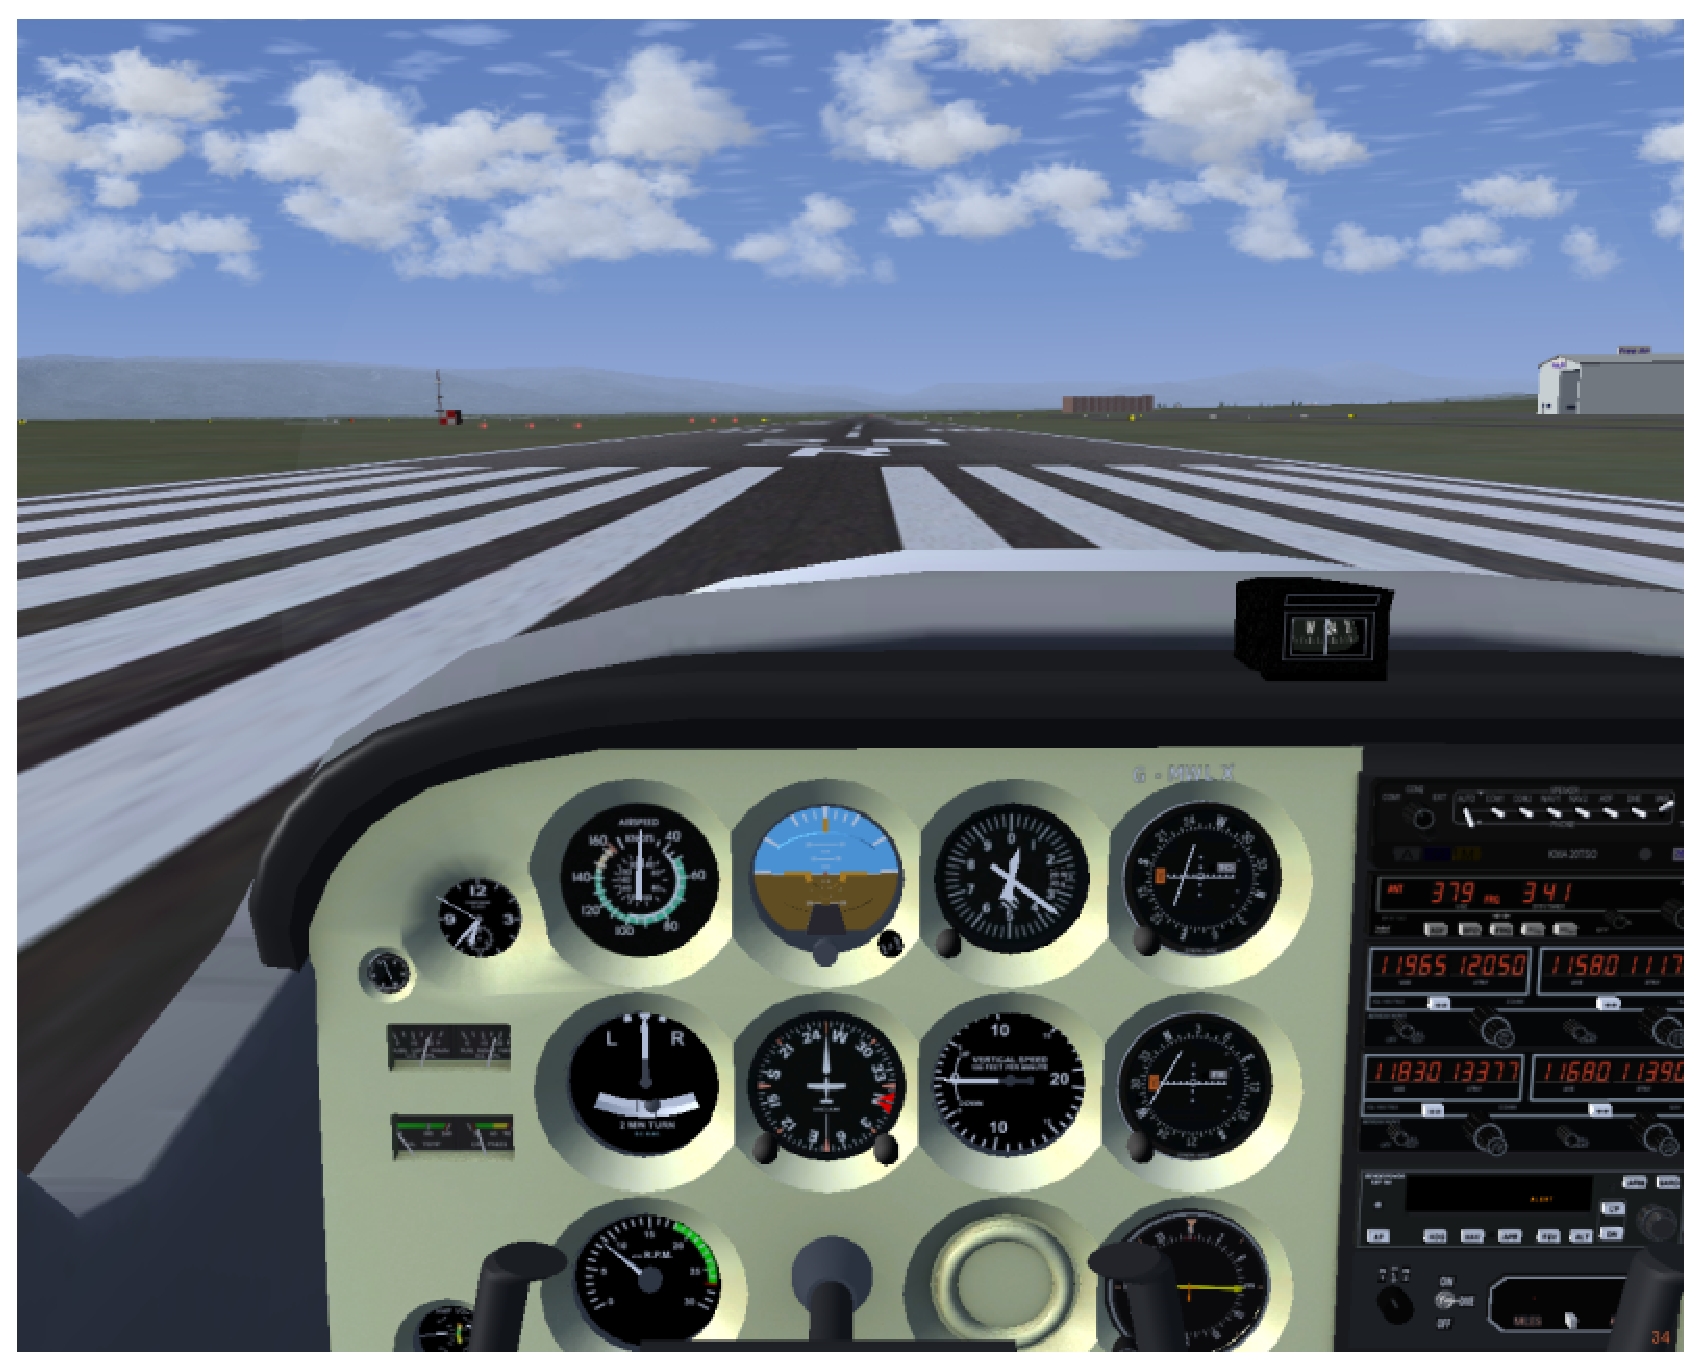
\includegraphics[clip,width=12.5cm]{panel3d}
}}

\smallskip
 \noindent
\iflanguage{english}{
Fig.\,6: \textit{The 3D cockpit of the Cessna 172.}
}{}
\iflanguage{french}{
Fig.\,6 : \textit{Le cockpit 3D d'un Cessna 172.}
}{}

\medskip

\iflanguage{english}{
Aircraft within \FlightGear{} can have both a 2-dimensional instrument panel
and a 3-dimensional cockpit. The 3-dimensional cockpit provides a much
more realistic pilot-eye view, but can be difficult to read with small
monitors.

The default Cessna 172P (c172p) has both a 3-dimensional and 2-dimensional
cockpit. The 3-dimensional cockpit is activated by default when you start
\FlightGear{}, but you can overlay the 2-dimensional instrument panel by
selecting \texttt{View->Display Options->Show 2D Panel} from the menu, or pressing the ``P'' key.

All panel levers and knobs can be operated with the mouse. To change a
control, just click with the left/middle mouse button on the
corresponding knob/lever. For controls that have a range of positions,
use the middle mouse button for larger adjustments. In general, clicking
on the right side of a control will increase the value, while clicking the left side
of the control will decrease the value.

Some instruments (particularly radios) also support use of a mouse scroll-wheel
to change values.
}{}
\iflanguage{french}{
Les a\'{e}ronefs au sein de \FlightGear{} peuvent avoir \`{a} la fois un tableau de bord \`{a} deux dimensions
et un cockpit \`{a} trois dimensions. Le cockpit \`{a} trois dimensions offre une vue beaucoup plus r\'{e}aliste, comme
si on \'{e}tait \`{a} la place du pilote, mais la lecture du tableau de bord peut \^{e}tre difficile avec des moniteurs de
dimensions r\'{e}duites.

Le Cessna 172P par d\'{e}faut (c172p) dispose \`{a} la fois d'un cockpit \`{a} deux et trois dimensions.
Le cockpit \`{a} 3 dimensions est activ\'{e} par d\'{e}faut lorsque vous d\'{e}marrez \FlightGear{}, mais vous pouvez y substituer
le tableau de bord \`{a} deux dimensions en choisissant \texttt{Affichage->Options d'affichage->Show 2D Panel} \`{a} partir du menu,
ou en appuyant sur la touche ``P''.

Tous les boutons et leviers peuvent \^{e}tre actionn\'{e}s avec la souris. Pour changer une commande, cliquez simplement avec
le bouton gauche/milieu sur le levier/bouton en question. Pour les commandes qui ont une large gamme de positions, utilisez le
bouton du milieu de la souris pour des ajustements plus grands. En g\'{e}n\'{e}ral, un clic sur le c\^{o}t\'{e} droit de la commande
augmentera sa valeur, alors qu'un clic sur le c\^{o}t\'{e} gauche la diminuera.

Certains instruments (en particulier les radios) supportent \'{e}galement l'utilisation de la molette de la souris pour l'ajustement
de leurs valeurs.
}{}

%%%%%%%%%%%%%%%%%%%%%%%%%%%%%%%%%%%%%%%%%%%%%%%%%%%%%%%%%%%%%%%%%%%%%%%%%%%%%%%%
%%%%%%%%%%%%%%%
\iflanguage{english}{
\section{The Head Up Display\index{head up display}}
}{}
\iflanguage{french}{
\section{Le collimateur t\^{e}te haute (\textit{Head Up Display, HUD})\index{head up display}}
}{}
%%%%%%%%%%%%%%%%%%%%%%%%%%%%%%%%%%%%%%%%%%%%%%%%%%%%%%%%%%%%%%%%%%%%%%%%%%%%%%%%
%%%%%%%%%%%%%%%

\iflanguage{english}{
\FlightGear{} also provides a \Index{HUD} (\textbf{H}ead \textbf{U}p
\textbf{D}isplay) \index{head up display}. HUDs are generally found in military
aircraft and some very advanced jets. However, \FlightGear{} also allows you
to use a HUD on many GA aircraft. To activate the HUD, press `h'.

The \Index{HUD} shown in Fig.\,7 displays all main flight parameters of the
plane. In the center you find the \Index{pitch indicator} (in degrees) with the
\Index{aileron indicator} above and the \Index{rudder indicator} below. A
corresponding scale for the elevator\index{elevation indicator} can be found
to the left of the pitch scale along with a pitch trim indicator. On the bottom
there is a simple \Index{turn indicator}.

There are two scales at the extreme left: The inner one displays the \Index{speed}
 (in kts) while the outer one indicates position of the \Index{throttle}.
The two scales on the extreme right display your \Index{height} - the left one
shows the height above ground while the right of it displays height above sea-level,
both being displayed in feet.

Besides this, the \Index{HUD} delivers some additions information. On the upper
left you will find date and time, along with your current position, in \Index{latitude}
and \Index{longitude}.

You can change color of the \textbf{HUD} using the ``H'' or ``'h''  key.
Pressing the toggle ``i/I'' minimizes/maximizes the HUD.
}{}
\iflanguage{french}{
\FlightGear{} fournit \'{e}galement un collimateur t\^{e}te haute ou \Index{HUD} (\textit{\textbf{H}ead \textbf{U}p \textbf{D}isplay}) \Index{HUD} \index{head up display}. On trouve g\'{e}n\'{e}ralement les HUD sur les a\'{e}ronefs
militaires et sur quelques avions \`{a} r\'{e}action modernes. Cependant, \FlightGear{} vous permet \'{e}galement
d'utiliser le HUD sur de nombreux a\'{e}ronefs de l'aviation g\'{e}n\'{e}rale. Pour activer le HUD, appuyez sur `h'.

Le \Index{HUD}, pr\'{e}sent\'{e} \`{a} la Fig.\,7 affiche tous les principaux param\`{e}tres de vol de l'a\'{e}ronef.
Au centre, vous trouvez l'indicateur d'\Index{assiette} (en degr\'{e}s) avec l'\Index{indicateur des ailerons} au-dessus
et l'\Index{indicateur de la gouverne de direction} dessous. Une \'{e}chelle correspondante pour la \index{gouverne de profondeur}
peut \^{e}tre trouv\'{e} \`{a} gauche de l'indicateur d'\'{e}chelle avec un indicateur de \textit{trim}. En bas se trouve un simple
\Index{indicateur de taux de virage}.

Il y a deux \'{e}chelles \`{a} l'extr\^{e}me gauche : celle qui est \`{a} l'int\'{e}rieur indique la \Index{vitesse}
(en noeuds) alors que celle \`{a} l'ext\'{e}rieur indique la position de la \Index{manette des gaz}.
Les deux \'{e}chelles \`{a} l'extr\^{e}me droite affichent votre \Index{altitude} - celle de gauche indique l'altitude au-dessus
du sol, alors que celle de droite indique l'altitude au-dessus du niveau de la mer, les deux \'{e}tant indiqu\'{e}es en pieds.

Enfin, le \Index{HUD} indique deux informations compl\'{e}mentaires. Dans le coin sup\'{e}rieur gauche vous aurez la date et l'heure,
ainsi que votre position actuelle en \Index{latitude} et \Index{longitude}.

Vous pouvez modifier la couleur du \textbf{HUD} en utilisant les touches ``H'' ou ``'h''. Un appui sur la touche ``i/I'' minimise/agrandit le HUD.
}{}

\medskip

 \centerline{\fbox{
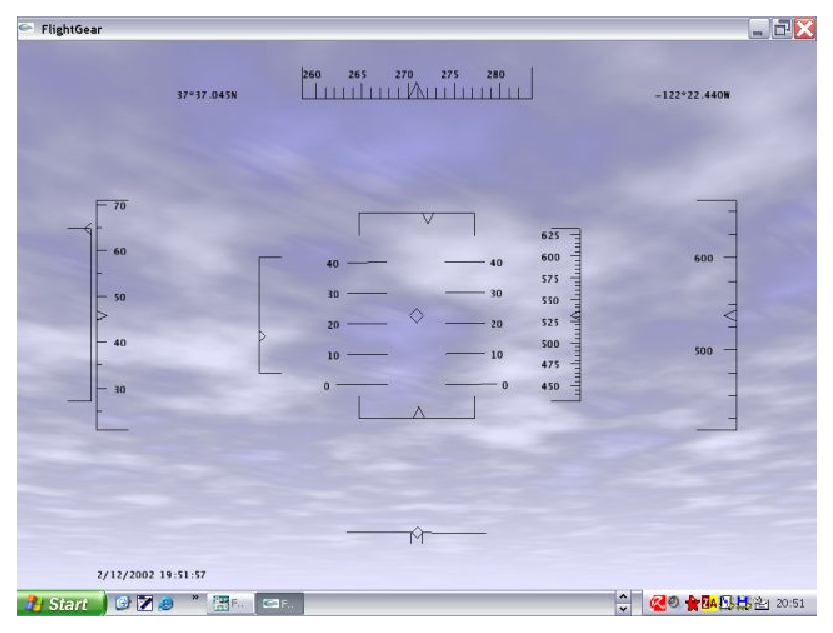
\includegraphics[clip,width=12.5cm]{hud2}
}}

\smallskip
 \noindent
\iflanguage{english}{
Fig.\,7: \textit{The HUD, or Head Up Display.}
}{}
\iflanguage{french}{
Fig.\,7 : \textit{Le collimateur t\^{e}te haute, ou HUD (Head Up Display).}
}{}
\medskip

%% Revision 0.00  1998/09/08  michael
%% Initial revision for version 0.53.
%% Revision 0.01  1998/09/20  michael
%% several extensions and corrections, added Fig.1.
%% revision 0.10  1998/10/01  michael
%% final proofreading for release
%% revision 0.11  1998/11/01  michael
%% Complete revision of keyborad controls, interesting places
%% revision 0.12  1999/03/07  michael
%% Corrected rudder key
%% revision 0.20  1999/06/04  michael
%% HUD completely rewritten, added panel section with picture, and menu section
%% updated keystrokes
%% revision 0.3 2000/04/20 michael
%% again updated and added keystrokes
%% revised menu entries
%% picture of new panel and re-written panel section
%% added mouse control section
%% Updated many keys, notably autopilot related, added two new tables
%% revision 0.4 2001/05/12 michael
%% updated/added many keystrikes, updated/added panel description
%% (radio stack etc.), new panel pic, panel before HUD now
%% short description of VOR/NDB
%% revision 0.41 2001/01/01 michael
%% added section on flight school material
%% added hints to user configurable *.xml files
%% revision 0.5 2002/01/01 michael
%% revised all changed keybindings now mostly read off of keyboard.xml
%% restructured tables more logically and put into separate files
%% for inclusion in Short Reference
%% New panel picture and revised descirption of panel according to new features
%% New HUD picture
%% revision 0.6 2002/09/05 michael
%% Several corrections/tweaks in plus renumbering of tables
%% Tweaks in menu entries
%% Added 3D cockpit picture
%% Changing numbers in radios
%% Added new menu items, swapped over 3D and 2-D pictures, as 3D cockpit is
%%  now the default
%% Revision 18/10/08: Numerous changes to improve readability, correct spelling errors etc.
%% Revision 8/3/09: Improved description of mouse modes.
%% Revision 26/12/09: Re-organization, move panel description to tutorial, update menu items.
